% Shadings (axial, radial, ball), transparency, a fading-free opacity group.
\documentclass{article}
\usepackage{tikz}
\begin{document}
Shadings and transparency.

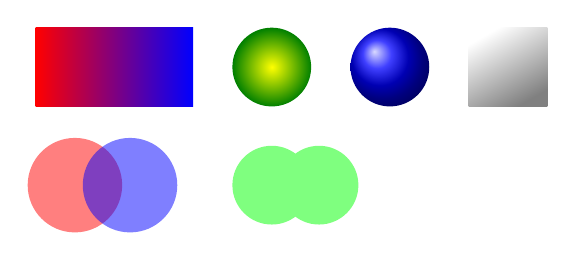
\begin{tikzpicture}
  \shade[left color=red, right color=blue] (0,0) rectangle (2,1);
  \shade[inner color=yellow, outer color=green!50!black] (3,0.5) circle (0.5);
  \shade[ball color=blue] (4.5,0.5) circle (0.5);
  \shade[top color=white, bottom color=gray, shading angle=30] (5.5,0) rectangle (6.5,1);
  \fill[red, opacity=0.5] (0.5,-1) circle (0.6);
  \fill[blue, fill opacity=0.5] (1.2,-1) circle (0.6);
  \begin{scope}[transparency group, opacity=0.5]
    \fill[green] (3,-1) circle (0.5); \fill[green] (3.6,-1) circle (0.5);
  \end{scope}
\end{tikzpicture}
\end{document}
